\chapter{Search Strategy}
\label{chap:Strategy}

\section{General Approach}
\label{sec:Strategy/general}

Candidate events in this search must have a total of at least three leptons, each of which can be either an electron or a muon. We classify multilepton events into search channels on the basis of the number of leptons, lepton flavor, lepton relative charges, charge and flavor combinations, and other kinematic quantities described below.

We classify each event in terms of the maximum number of opposite-sign same-flavor (OSSF) dilepton pairs that can be made by using each lepton only once. For example, both $\mu^+\mu^-\mu^-$ and $\mu^+\mu^-e^-$ are OSSF1, $\mu^+\mu^+e^-$ is OSSF0, and $\mu^+\mu^-e^+e^-$ is OSSF2. We denote a lepton pair of different flavors as $\ell\ell^\prime$.

We classify events as containing a leptonically-decaying \Z if at least one OSSF pair has $m_{\ell^+\ell^-}$ in the \Z mass window $91 \pm 10\,\GeV$. For $m_{\ell^+\ell^-}$ outside the \Z boson mass window, events are separated into bins below and above the \Z mass window. We refer to these three mass ranges as ``on-\Z'', ``below-\Z'', and ``above-\Z''.

In cases of ambiguity (such as $\mu^+\mu^-\mu^-$ with one pair below and one pair above \Z), we need to pick a specific pair. We compare two methods:
\begin{enumerate}
	\item Choose the pair whose invariant mass is closest to the \Z mass.
	\item Choose the pair closest to the \Z mass, with the additional condition that pairs above the \Z window are not considered if there is a pair below the \Z window (thus shifting events from above-\Z to below-\Z).
\end{enumerate}
Fig.~\ref{fig:app:Zbinning} shows that there is little difference between both approaches. Nevertheless, we take the second approach to achieve a more separative categorization of background, especially around the high end of the \Z window.
\begin{figure}
\begin{center}
	\begin{subfigure}[b]{.7\textwidth}
		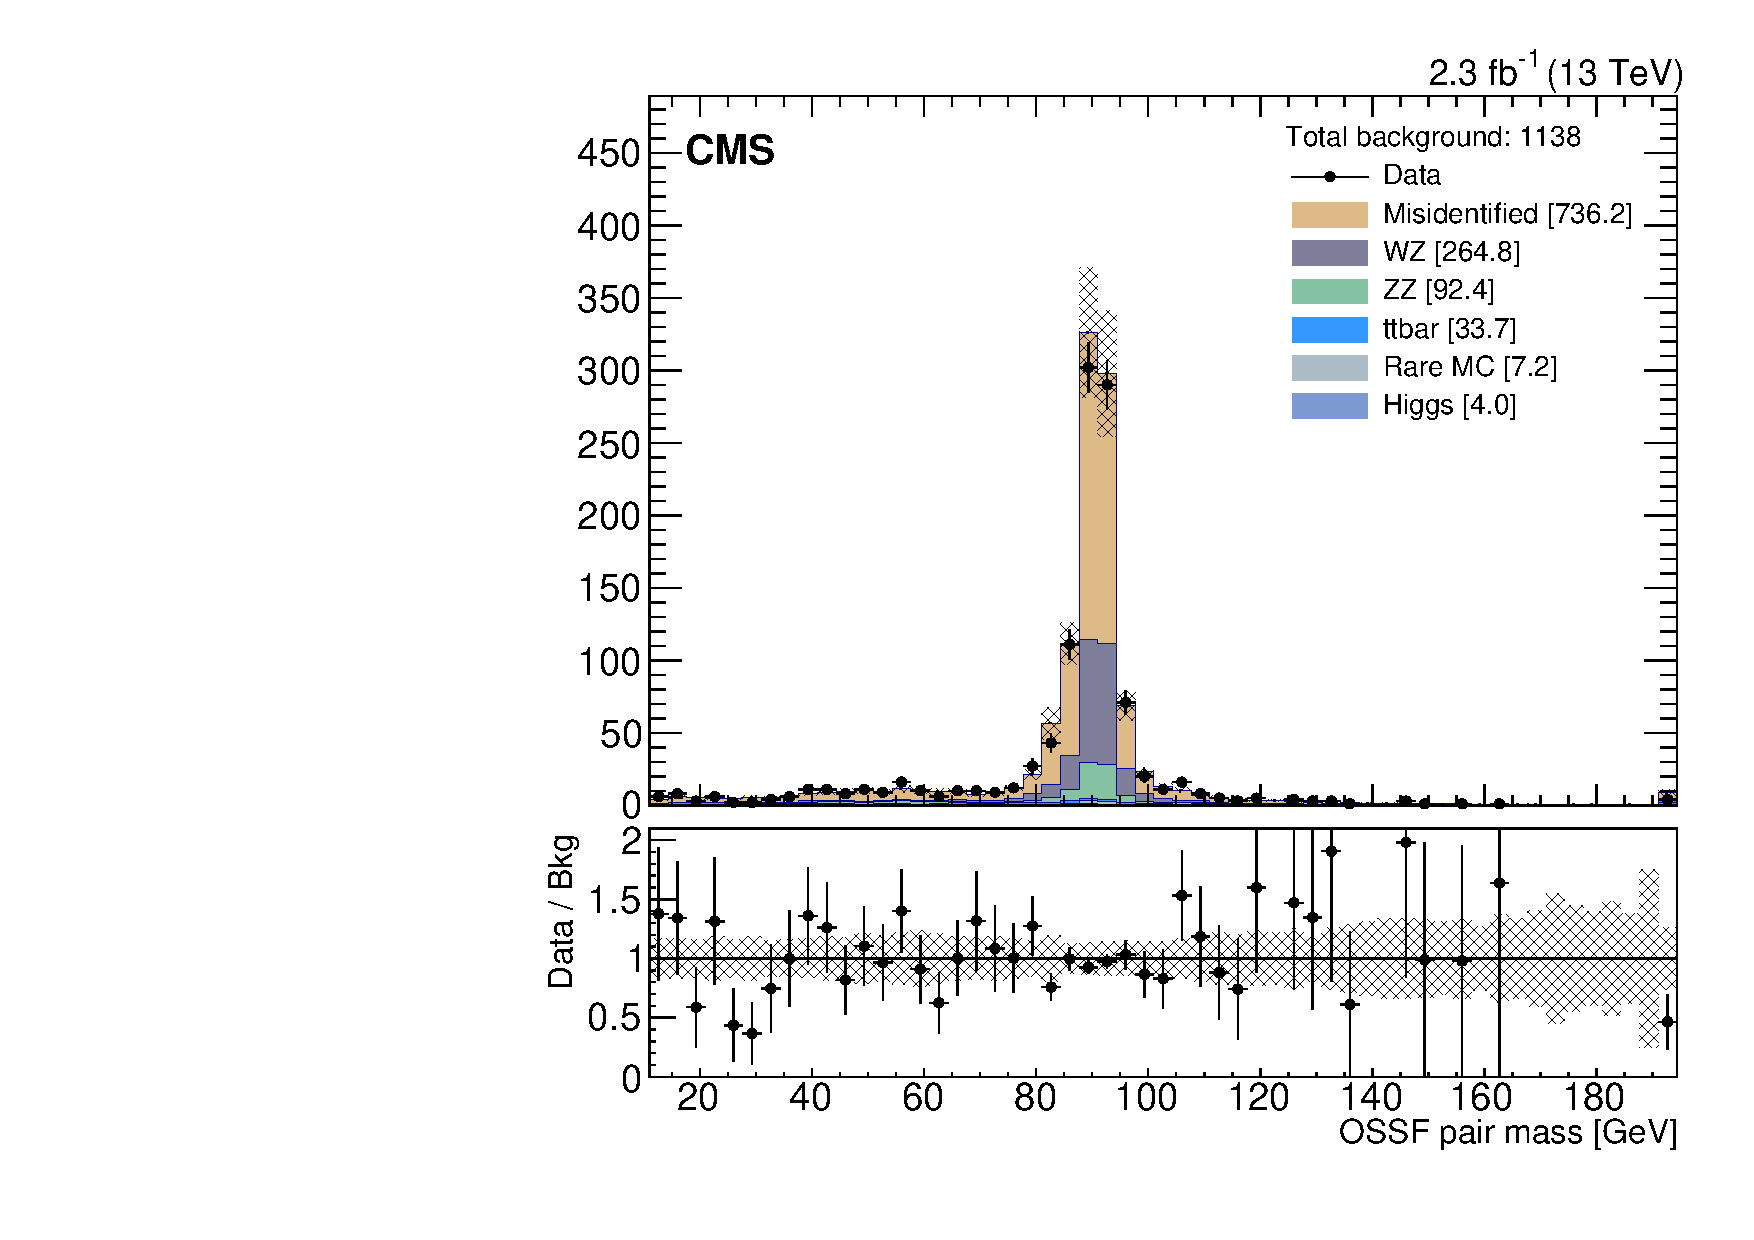
\includegraphics[width=\textwidth]{Strategy/Z_L3MET0to50_noAIC_OSSFCLOSEMLL}%
		\caption{method 1}
	\end{subfigure}
	\begin{subfigure}[b]{.7\textwidth}
		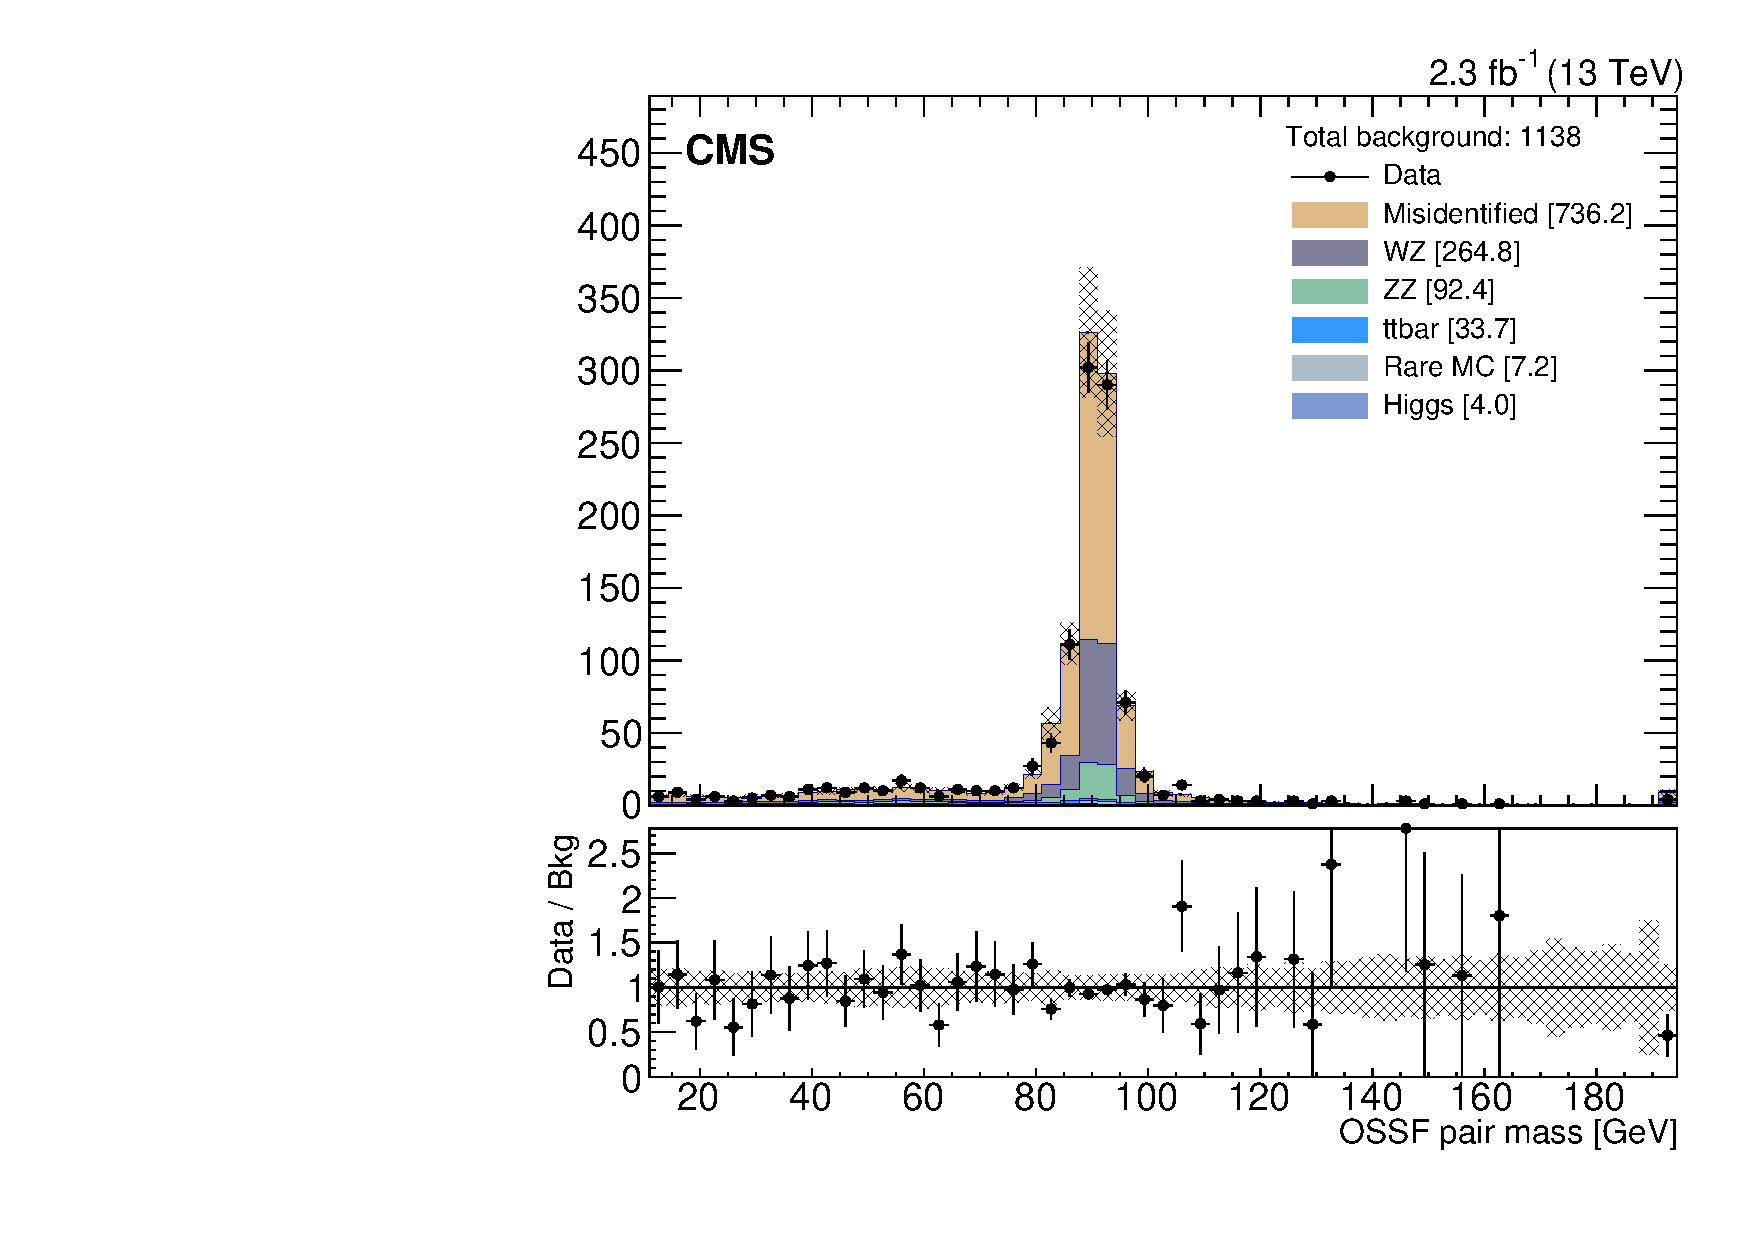
\includegraphics[width=\textwidth]{Strategy/Z_L3MET0to50_noAIC_MOSSF}
		\caption{method 2}
	\end{subfigure}
	\caption{$m_{\ell\ell}$ distribution in in the dilepton fake region (off-\Z, trilepton events with $m_{\ell\ell\ell}$ on \Z have been vetoed).
	\label{fig:app:Zbinning}}
\end{center}
\end{figure}

The most important multilepton background processes are \WZ, \Z or \ttbar events in which there is a misidentified lepton, and \ZZ production. In addition, there are various rare background processes like WWZ or $\ttbar\PW$. However, the level of SM background varies considerably across channels; for example, channels containing OSSF pairs suffer from larger backgrounds than do channels with OSSF0. Hence, all these charge combinations are considered as different channels.

%Backgrounds can be tamed by binning in appropriate quantities. Since the signal leptons have relatively high \pt and since in some decay modes there is missing transverse energy (\MET) from accompanying neutrinos, we find that binning in $L_\textrm{T} + \MET$, where $L_\textrm{T}$ is the scalar sum of the lepton \pt's, separates the signal from the background. We find that lepton \pt binning alone gives about 20\,\% worse signal-to-background ratios in the most sensitive signal regions.
%Additional separation is achieved through the on- and off-\Z binning described above.

\section{Signal Regions}
\label{sec:Optimization}

%The type-III seesaw signal comes both with 3 and 4 (or more) leptons as well as with and without OSSF pairs, which in turn may have an invariant mass that is compatible with \Z production. This lays the foundation for our binning scheme.

Backgrounds can be tamed by binning in appropriate quantities. Given the relatively high signal lepton momenta due to the large masses of the parent particles, cutting on $L_\textrm{T}$, the scalar lepton \pt sum, may be a good idea. This is especially true for decay modes like $\Sigma^\pm \to \ell^\pm \Z \to \ell^\pm ~ \ell^{\prime \pm} \ell^{\prime \mp}$ where the heavy fermion mass is transformed into the lepton momenta. However, such an $L_\textrm{T}$ cut acts at the expense of the signal efficiency in other modes like $\Sigma^0 \to \PH \nu \to \PW\PW\nu$, where lepton \pt's are somewhat lower because the intermediate bosons may be off-shell, and the neutrinos carry away some of the momentum that appears as missing transverse energy (\MET). However, we can still achieve high efficiency by using $L_\textrm{T} + \MET$ instead, which we found suitable for signal selection for both of the described channel types (Fig.~\ref{fig:Optimization2}). The background rejection effectiveness of this variable is shown in Fig.~\ref{fig:Optimization}. We find that lepton \pt binning alone gives about 20\,\% worse signal-to-background ratios in the most sensitive signal regions.

\begin{figure}
\begin{center}
	\begin{subfigure}[b]{.7\textwidth}
		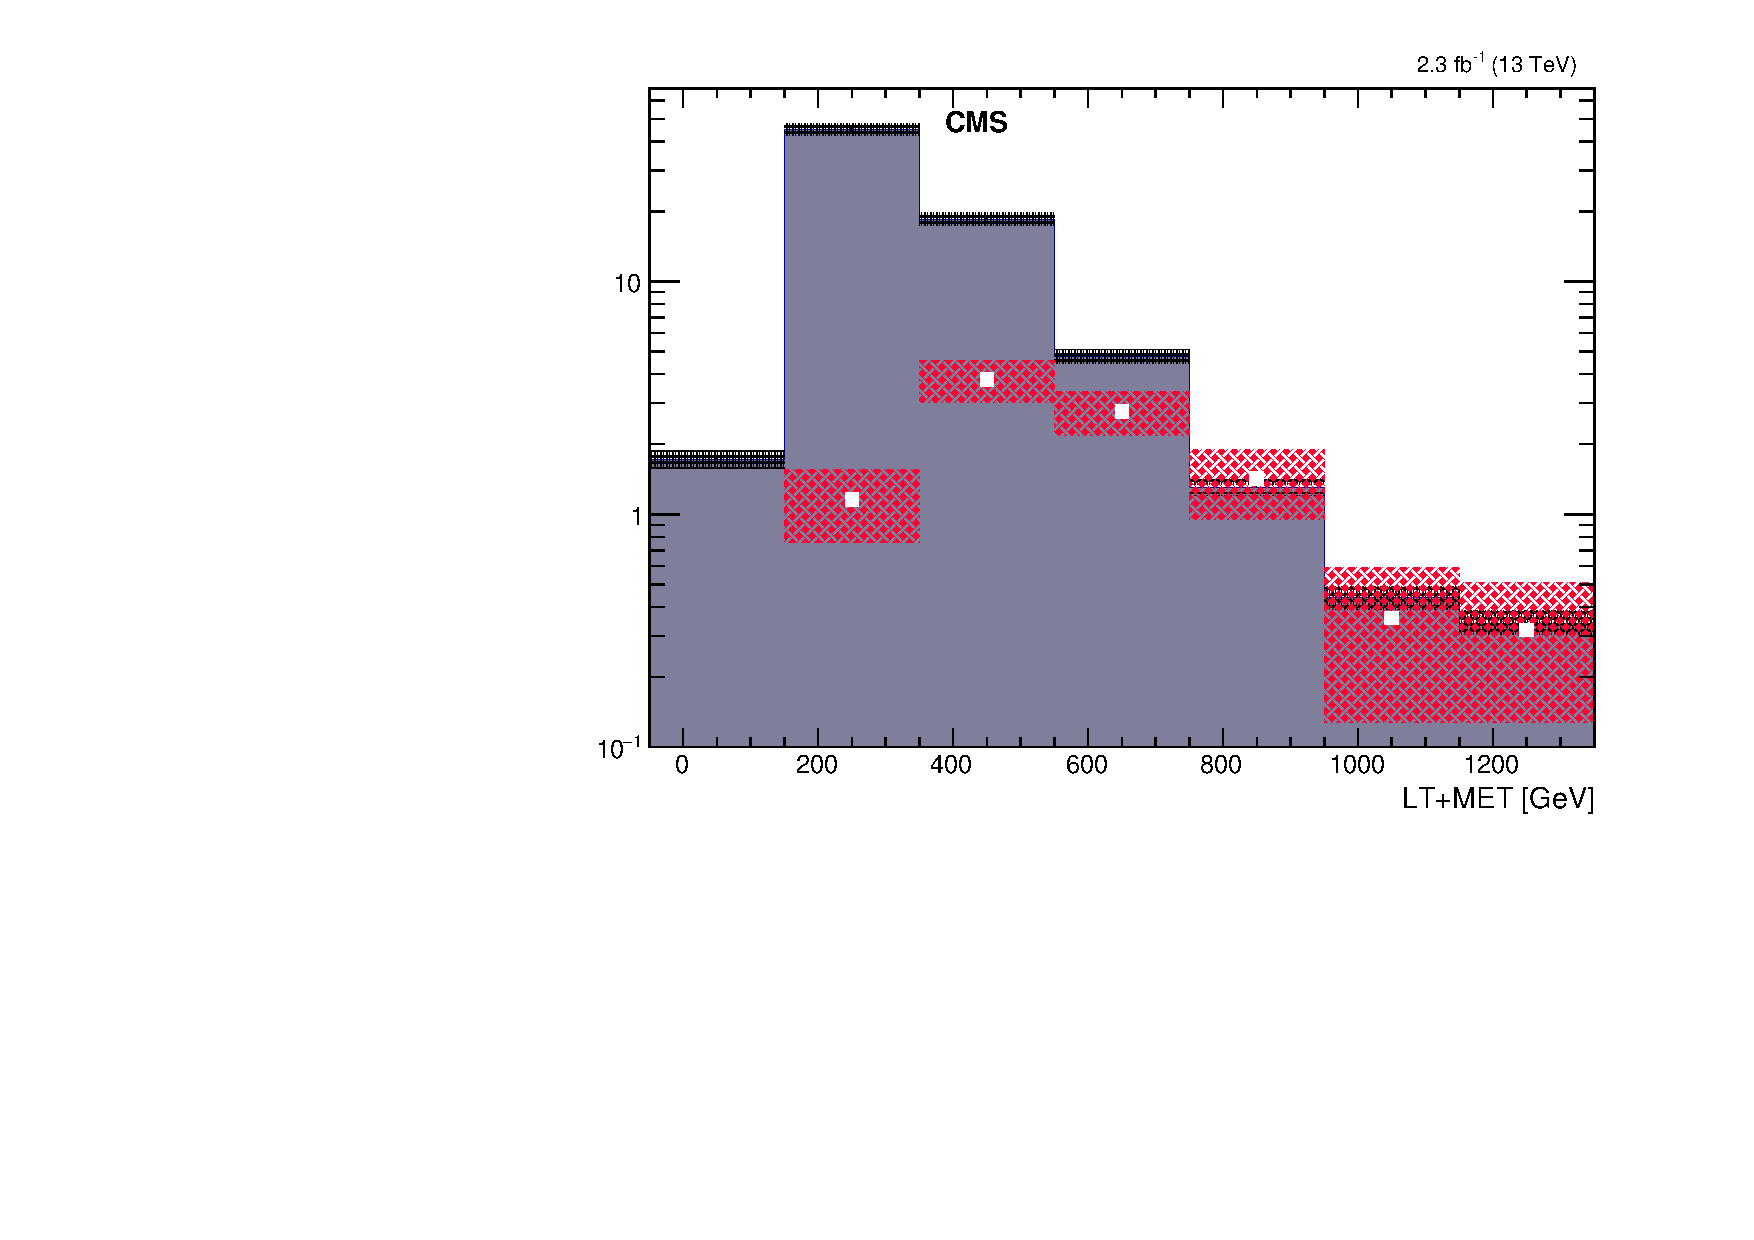
\includegraphics[width=\textwidth]{Strategy/LT+MET_tr+w+vltr0wl}
		\caption{$\Sigma^+ \to \PW^+ \nu, \Sigma^0 \to \PW^\pm \ell^\mp$}
	\end{subfigure}
	\begin{subfigure}[b]{.7\textwidth}
		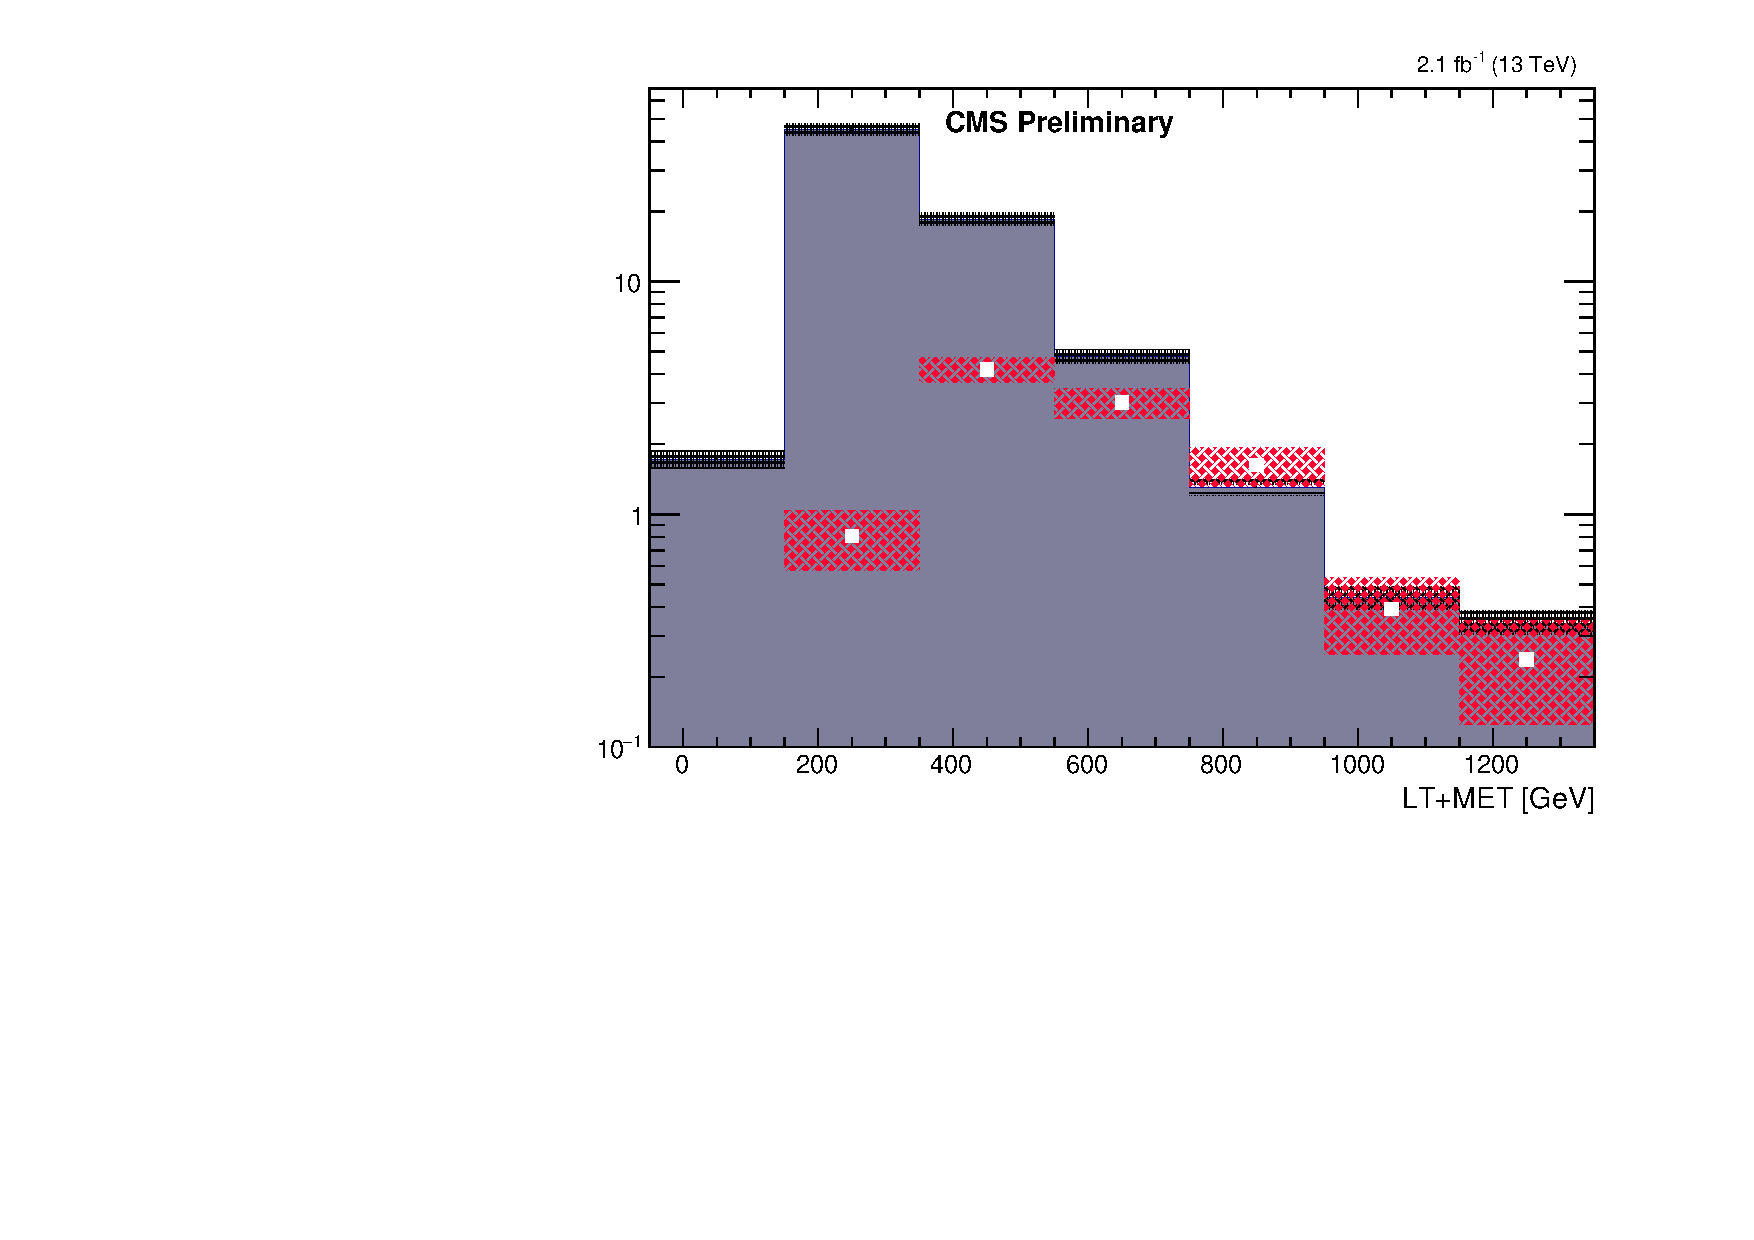
\includegraphics[width=\textwidth]{Strategy/LT+MET_tr+zl+tr-zl-}
		\caption{$\Sigma^+ \to Z \ell^+, \Sigma^- \to Z \ell^-$}
	\end{subfigure}
	\caption{$L_\textrm{T} + \MET$ shape for two different production and decay modes at $m_\Sigma = 340\,\GeV$, with \WZ background. Signal normalization arbitrary (for illustration purposes only).
	\label{fig:Optimization2}}
\end{center}
\end{figure}

\begin{figure}
\begin{center}
	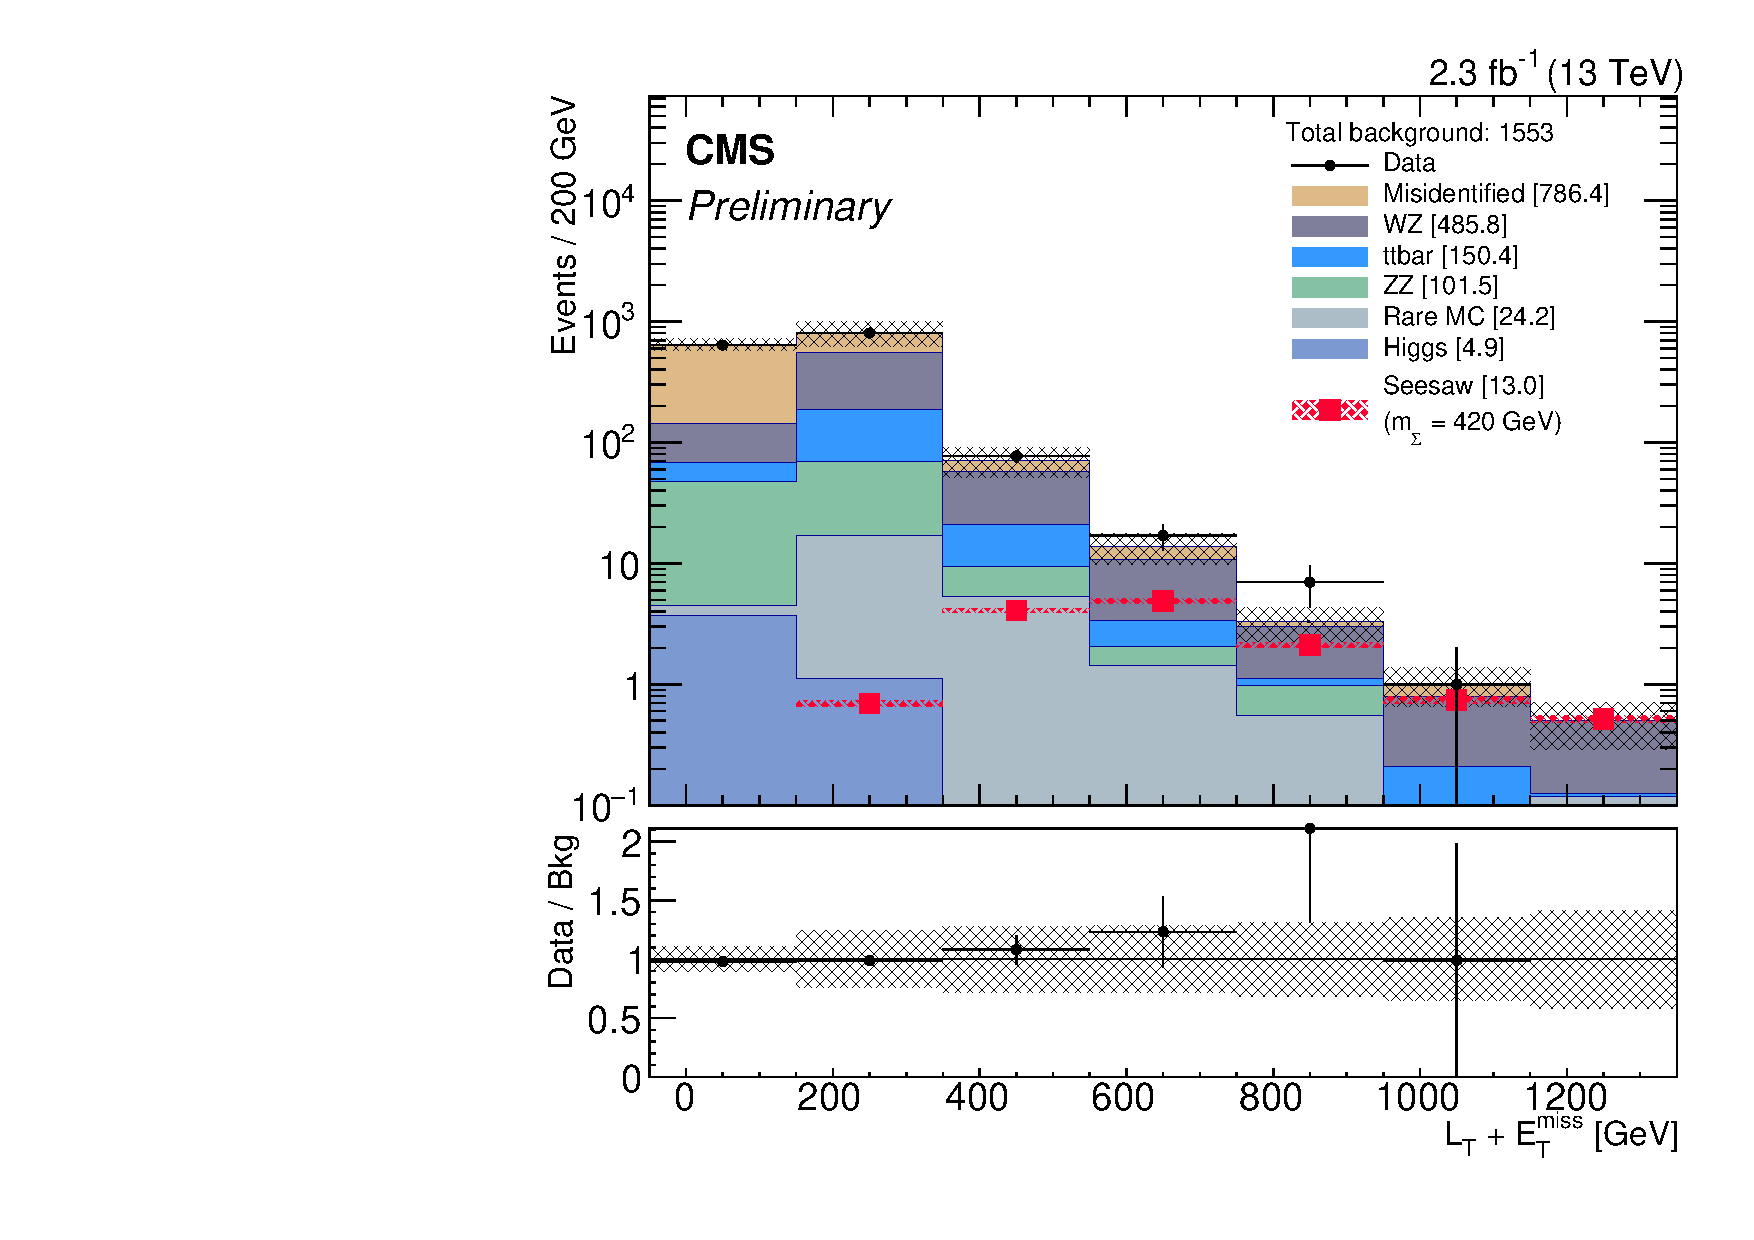
\includegraphics[width=.7\textwidth]{Strategy/LT+MET}
	\caption{$L_\textrm{T} + \MET$ distribution after event selection cuts from Sec.~\ref{sec:Selection}, to illustrate the signal separation power of this variable (last bin includes overflow). Backgrounds are described in Chapter~{\ref{chap:Backgrounds}}. The signal ($m_\Sigma = 420\,\GeV$, sum of all production and decay modes) is shown as white square dots with a pink hashed uncertainty band. The background uncertainty is specified by the gray band. Uncertainty bands include both statistical and systematic uncertainties. Numbers in square brackets denote the number of events contributed by each process.
	\label{fig:Optimization}}
\end{center}
\end{figure}

The optimum requirement on $L_\textrm{T} + \MET$ depends on the mass of the heavy fermions. In order to separate the signal as well as possible from the background, we categorize the data in bins of $L_\textrm{T} + \MET$, regardless of the particle mass. We use 4 bins of width 200\,\GeV starting at 350\,\GeV, plus an overflow bin. Below 350\,\GeV, the amount of signal is insignificant in comparison to the background.

We remove any overlap with background control regions by explicitly vetoing the control region selections. Furthermore, we discard the below-\Z trilepton region and the four-lepton region without an OSSF pair because, with the given amount of luminosity, they contain a neglibile amount of signal and thus do not contribute to the sensitivity.

As a result, we have four $L_\textrm{T} + \MET$ distributions, depending on the lepton properties: 3 leptons without OSSF pair, 3 leptons with OSSF pair on-\Z, 3 leptons with OSSF pair above-\Z, and 4 leptons with at least one OSSF pair. Each distributions begins at 350\,\GeV and reaches to 1150\,\GeV in steps of 200\,\GeV. We add an overflow bin for $L_\textrm{T} + \MET > 1150\,\GeV$ so that that there are five bins per distribution. The resulting set of 20 signal regions is described in Table~\ref{tab:SR}.

\begin{table}
\centering
\caption{Signal Regions. Overlap with control regions removed everywhere.} \label{tab:SR}
\begin{tabular}{c l c }
\hline\hline
$n_\textrm{leptons}$ & OSSF pair & $L_\textrm{T} + \MET$ [GeV]\\
\hline
3 & & \\
 & none & \multirow{3}{*}{\rotatebox{9}{350..1150 in steps of 200, plus overflow}} \\
 & on-\Z & \\
 & above-\Z & \\
\hline
$\geq 4$ & $\geq 1$ & 350..1150 in steps of 200, plus overflow \\
\end{tabular}
\end{table}
